\input ../SlidePreamble
\input ../preamble


\begin{document}

{\Huge

  \centerline{\bf TTIC 31230, Fundamentals of Deep Learning}
  \bigskip
  \centerline{David McAllester, Autumn 2023}
  \vfill
  \vfil
  \centerline{The Mathematics of Diffusion Models}
  \vfill
  \centerline{McAllester, arXiv January 2023}
    \vfill
  \vfill

\slidetwo{Denoising Diffusion Probabilistic Models (DDPM)}{Ho, Jain and Abbeel, June 2020}

\centerline{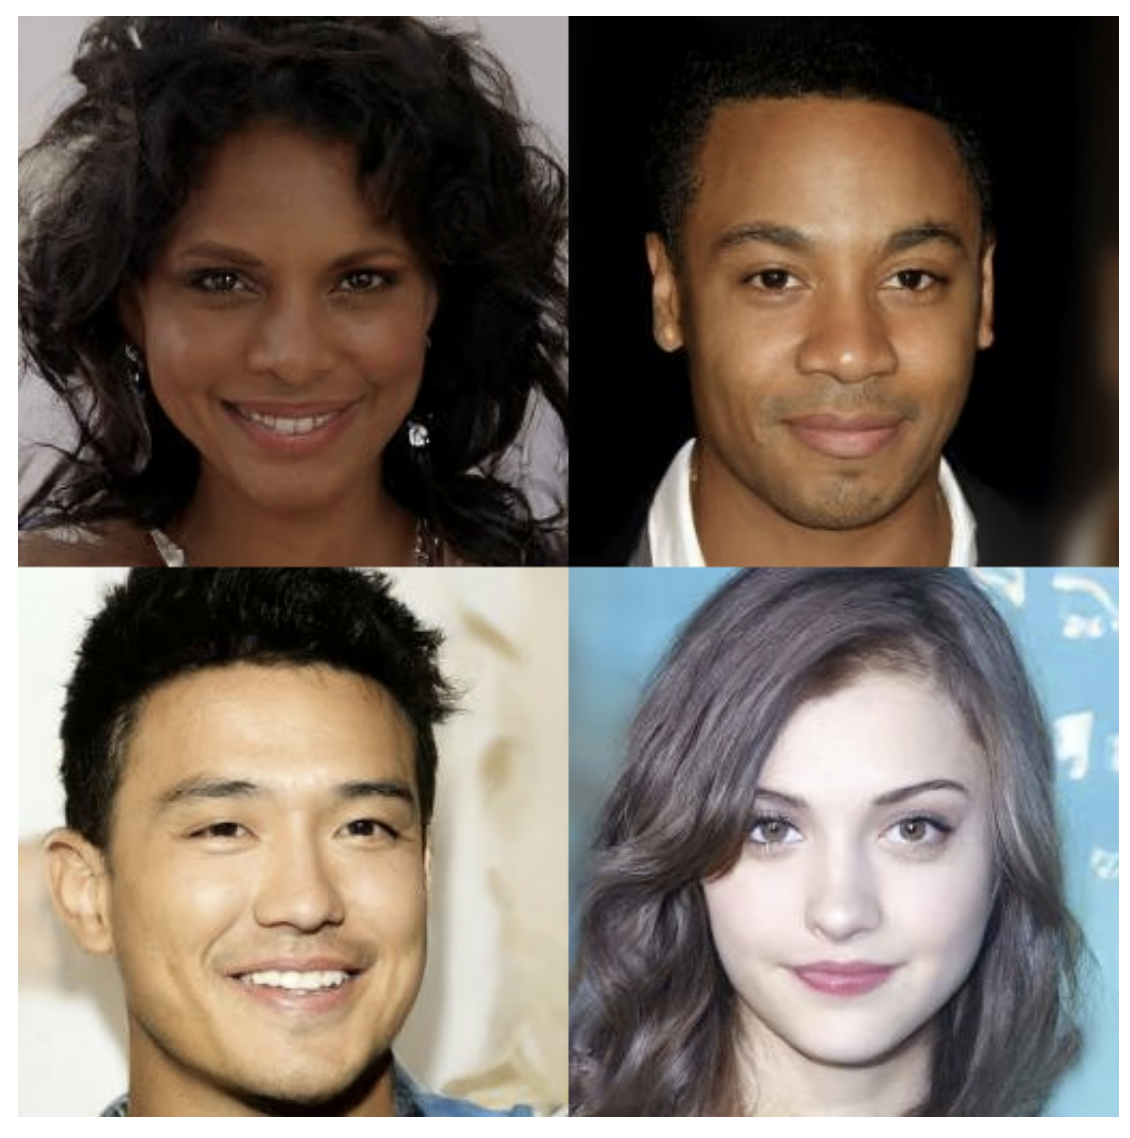
\includegraphics[width = 4in]{\images/DiffCeleb}}

\slide{The Diffusion SDE}
\centerline{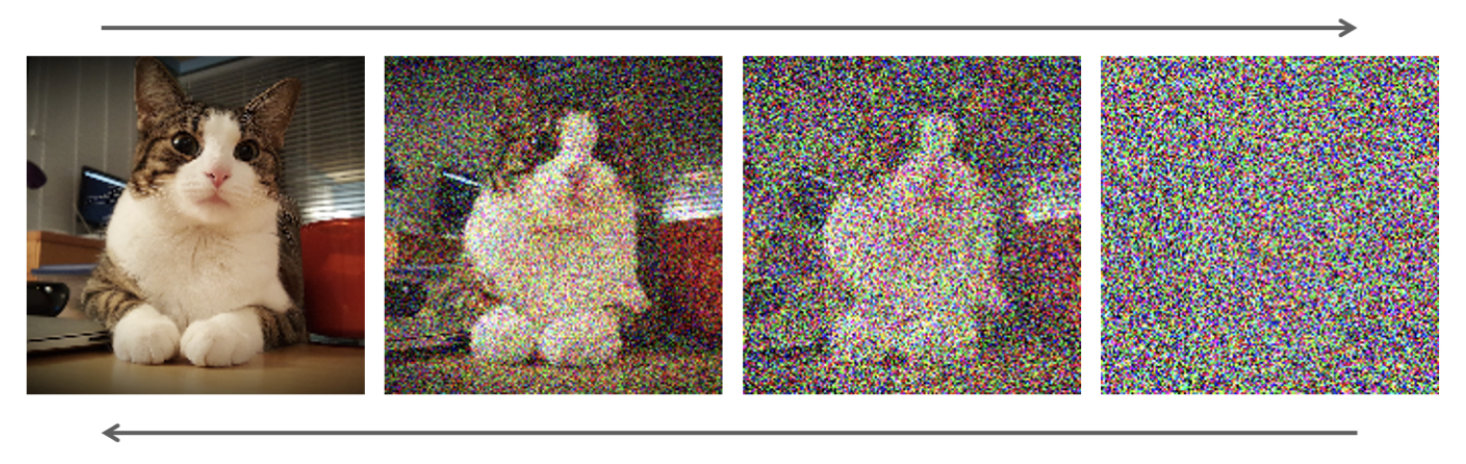
\includegraphics[width = 2in]{\images/DiffSequence}}

Consider a discrete time process $z(0),z(\Delta t),z(2\Delta t),z(3\Delta t),\ldots$
{\huge
\begin{eqnarray*}
  z(0) & = & y,\;\;\;y \sim \pop(y) \\
  \\
  z(t+\Delta t) & = & z(t) + \sqrt{\Delta t}\; \epsilon,\;\;\;\epsilon \sim {\cal N}(0,I)
\end{eqnarray*}
}

A sum of two Gaussians is a Gaussian whose {\bf variance} is the sum of the two variances.
$$z(t+n\Delta t) = z(t) + \sqrt{n\Delta t}\; \epsilon,\;\;\;\epsilon \sim {\cal N}(0,I)$$
Here $\sqrt{n \Delta t}$ is the {\bf standard deviation} of the added noise.

\slide{SDE Notation}
In these slides $\epsilon$ will always be a random variable drawn from ${\cal N}(0,I)$.

\vfill
This correspods to ``$dB$'' in the more standard way of writing SDEs.

{\huge
\begin{eqnarray*}
  z(t+\Delta t) & = & z(t) + \mu(z,t)\Delta t + \sigma(z,t)\epsilon\sqrt{\Delta t} \\
  \\
  dz & = & \mu(z,t)dt + \sigma(z,t)dB
\end{eqnarray*}
}

\vfill
While the expression in terms of $\Delta t$ is more verbose, it seems clearer to me.

\slide{The Diffusion SDE}
The stochastic differential equation is the limit as the discrete step size $\Delta t$ goes to zero.

\vfill
For the diffusion process (Brownian motion) we have

{\huge
\begin{eqnarray}
  z(0) & = & y,\;\;\;y \sim \pop(y) \nonumber \\
  \nonumber \\
  z(t+\Delta t) & = & z(t) + \epsilon\sqrt{\Delta t} \label{forward}
\end{eqnarray}
}



\vfill
For diffusion we get that (\ref{forward}) holds for all $t$ and $\Delta t$.

\slide{Probability Notation}

In these slides unsubscripted probability notation, such as

\vfill
$$P(z(t+\Delta t)|z(t)),$$

\vfill
or a conditiional expectation such as

\vfill
$$E[f(y)|z(t)] = E_{y \sim P(y|z_t)}[f(y)],$$

\vfill
refer the joint probability distribution on $y$ and the (continuous) function $z(t)$
defined by the diffusion process.

\slide{Reverse-Time Probabilities}

In the limit of small $\Delta t$ it is possible to derive the following.

\vfill
\begin{eqnarray*}
  p(z(t - \Delta t)|z(t),y) & = & {\cal N}\left(\begin{array}{l}z(t) + \frac{\Delta t(y - z(t))}{t},\;\; \Delta t I\end{array}\right) \\
  \\
  \\
  p(z(t - \Delta t)|z(t)) & = & {\cal N}\left(\begin{array}{l} z(t) + \frac{\Delta t(E[y|t,z(t)] - z(t))}{t}, \;\; \Delta t I\end{array}\right)
\end{eqnarray*}


\slide{The Reverse-Diffusion SDE}

$$p(z(t - \Delta t)|z(t)) = {\cal N}\left(\begin{array}{l} z(t) + \frac{\Delta t(E[y|t,z(t)] - z(t))}{t}, \Delta t I\end{array}\right)$$

\vfill
This equation defines a reverse-diffusion SDE which we can write as

{\huge
$$z(t - \Delta t) = z(t) + \left(\frac{E[y|t,z(t)] - z(t)}{t}\right)\Delta t + \sqrt{\Delta t} \epsilon,\;\;\epsilon \sim {\cal N}(0,I)$$
}

\slide{Estimating $E[y|t,z(t)]$}

$$z(t - \Delta t) = z(t) + \left(\frac{E[y|t,z(t)] - z(t)}{t}\right)\Delta t + \epsilon\sqrt{\Delta t},\;\;\epsilon \sim {\cal N}(0,I)$$

\vfill
We can train a denoising network $\hat{y}(t,z)$ to estimate $E[y|t,z(t)]$ using

\vfill
$$\hat{y}^* = \argmin_{\hat{y}} E_t \;E \;(\hat{y}(t,z) - y)^2$$

\vfill
Assuming universality

\vfill
$$\hat{y}^*(t,z) = E[y|t,z(t)]$$

\slide{Estimating $E[y|t,z(t)]$}
In practice it is better to train the denoising network on values of the same scale.

\vfill
If the population values are scaled so as to have scale 1, then the scale of $z(t)$ is $\sqrt{1+t}$.
$$\hat{y}^* = \argmin_{\hat{y}} E_{t,z(t)} \; (\hat{y}(t,z/\sqrt{1+t}) - y)^2$$

\vfill
We then have
$$E[y|t,z(t)] = \hat{y}^*(t,z/\sqrt{1+t}))$$


\slide{Computing Bits per Channel (or Perplexity)}

For any Markovian VAE we have

\vfill
{\Large
\begin{eqnarray}
  - \ln \pop(y) & = & - \ln\frac{P(z_N)P(z_{N-1}|z_N)\cdots P(z_1|z_2)P(y|z_1)}{P(z_N|y)P(z_{N-1}|z_N,y)\cdots P(z_1|z_2,y)} \nonumber\\
  \nonumber \\
  \nonumber \\
  H(y) & = & \left\{\begin{array}{l} E[KL(P(z_N|y),\;P(z_N))] \\ \\ + \sum_{i=2}^N  \; E[KL(P(z_{i-1}|z_i,y),\;P(z_{i-1}|z_i))] \\ \\ +\;E[\ln -P(y|z_1)] \end{array}\right. \label{Markov-eq} \\
  \nonumber\\
  \nonumber\\
  & \leq & \left\{\begin{array}{l} E[KL(P(z_N|y),\;P_\gen(z_N))] \\ \\ + \sum_{i=2}^N  \; E[KL(P(z_{i-1}|z_i,y),\;P_\gen(z_{i-1}|z_i))] \\ \\ E[- \ln P_\gen(y|z_1)] \end{array}\right. \;\;\;~\label{Markov-ELBO}
\end{eqnarray}
}

\slide{KL-Divergence}

{\huge
\begin{eqnarray*}
  H(y) & = & \left\{\begin{array}{l} E[KL(P(z_N|y),\;P(z_N))] \\ \\ + \sum_{i=2}^N  \; E[KL(P(z_{i-1}|z_i,y),\;P(z_{i-1}|z_i))] \\ \\ +\;E[\ln -P(y|z_1)] \end{array}\right.
  \end{eqnarray*}

\vfill
For two Gaussian distributions with the same isotropic covariance we have

\vfill
$$KL\left(\begin{array}{l}{\cal N}(\mu_1,\sigma^2 I), \\ {\cal N}(\mu_2,\sigma^2 I) \end{array}\right) = \frac{||u_1 -\mu_2||^2}{2\sigma^2}$$
}

\slide{KL-Divergence}
{\huge
\begin{eqnarray*}
  H(y) & = & \left\{\begin{array}{l} E[KL(P(z_N|y),\;P(z_N))] \\ \\ + \sum_{i=2}^N  \; E[KL(P(z_{i-1}|z_i,y),\;P(z_{i-1}|z_i))] \\ \\ +\;E[\ln -P(y|z_1)] \end{array}\right.
\end{eqnarray*}

\vfill
\begin{eqnarray*}
  p(z(t - \Delta t)|z(t),y) & = & {\cal N}\left(\begin{array}{l}z(t) + \frac{\Delta t(y - z(t))}{t},\;\; \Delta t I\end{array}\right) \\
  \\
  \\
  p(z(t - \Delta t)|z(t)) & = & {\cal N}\left(\begin{array}{l} z(t) + \frac{\Delta t(E[y|t,z(t)] - z(t))}{t}, \;\; \Delta t I\end{array}\right)
\end{eqnarray*}
}

\slide{KL-Divergences}
{\huge
\begin{eqnarray*}
  p(z(t - \Delta t)|z(t),y) & = & {\cal N}\left(\begin{array}{l}z(t) + \frac{\Delta t(y - z(t))}{t},\;\; \Delta t I\end{array}\right) \\
  \\
  \\
  p(z(t - \Delta t)|z(t)) & = & {\cal N}\left(\begin{array}{l} z(t) + \frac{\Delta t(E[y|t,z(t)] - z(t))}{t}, \;\; \Delta t I\end{array}\right)
\end{eqnarray*}

\vfill
\begin{eqnarray*}
  KL\left(\begin{array}{l}p(z(t-\Delta t)|z(t),y), \\p(z(t-\Delta  t)|z(t))\end{array}\right)
  & = & \left(\frac{||y-E[y|t,z(t)]||^2\Delta t^2}{2t^2\Delta t}\right) \\
  \\
  \\
  & =  & \left(\frac{||y-E[y|t,z(t)]||^2}{2t^2}\right) \Delta t
\end{eqnarray*}
}

\slide{KL-Divergences}
\begin{eqnarray*}
  H(y) & = & \left\{\begin{array}{l} E[KL(P(z_N|y),\;P(z_N))] \\ \\ + \sum_{i=2}^N  \; E[KL(P(z_{i-1}|z_i,y),\;P(z_{i-1}|z_i))] \\ \\ +\;E[\ln -P(y|z_1)] \end{array}\right.
  \\
  \\
  \\
  & = & \sum_{i = 2}^N  \left(\frac{||y-E[y|t,z(t)]||^2}{2t^2}\right) \Delta t + E\;[- \ln P(y|z_1)] \\
  & & \;\;\;\;\;\;\;\;\;\;\;\;\;\;\;\;\;t = i\Delta t
\end{eqnarray*}

\slide{KL-Divergences}
\begin{eqnarray*}
  H(y) - H(y|z_1) & = & \left\{\begin{array}{l} E[KL(P(z_N|y),\;P(z_N))] \\ \\ + \sum_{i=2}^N  \; E[KL(P(z_{i-1}|z_i,y),\;P(z_{i-1}|z_i))] \end{array}\right.
  \\
  \\
  & = & I[y,z_1] \\
  \\
  \\
  &\leq & 
  \\
  & = & \sum_{i = 2}^N  \left(\frac{||y-E[y|t,z(t)]||^2}{2t^2}\right) \Delta t + E\;[- \ln P(y|z_1)] \\
  & & \;\;\;\;\;\;\;\;\;\;\;\;\;\;\;\;\;t = i\Delta t
\end{eqnarray*}

\slide{Passing to the Integral}

\begin{eqnarray*}
H(y) & = & \left\{\begin{array}{l}\int_{t_0}^\infty dt \;\; E_{z(t)|y}\;\left[\frac{||y - E[y|t,z(t)]||^2}{2t^2}\right] \\ \\ + \;E_{z(t_0)|y}[-\ln p(y|z(t_0))]\end{array}\right. \\
\\
\\
  H(y) & = & \left\{\begin{array}{l}\int_{t_0}^\infty dt \;\; E_{y,z(t_0)}\;\left[\frac{||y - E[y|t,z(t)]||^2}{2t^2}\right] \\ \\ +\;H(y|z(t_0))\end{array}\right.
\end{eqnarray*}

\slide{Mutual Information}

{\huge
\begin{eqnarray*}
  H(y) & = & \left\{\begin{array}{l}\int_{t_0}^\infty dt \;\; E_{y,z(t_0)}\;\left[\frac{||y - E[y|t,z(t)]||^2}{2t^2}\right] \\ \\ +\;H(y|z(t_0))\end{array}\right. \\
  \\
  \\
  H(y) - H(y|z(t_0)) & = & \int_{t_0}^\infty dt \;\; E_{y,z(t_0)}\;\left[\frac{||y - E[y|t,z(t)]||^2}{2t^2}\right] \\
  \\
  \\
  I(y,z(t_0)) & = & \int_{t_0}^\infty dt \;\; E_{y,z(t_0)}\;\left[\frac{||y - E[y|t,z(t)]||^2}{2t^2}\right] 
\end{eqnarray*}

\vfill
This is the information minimum mean squared error relation (I-MMSE) relation [Guo et al. 2005].
}

\slide{Computing Bits per Channel}

{\huge
\begin{eqnarray*}
  I(y,z(t_0)) & = & \int_{t_0}^\infty dt \;\; E_{y,z(t_0)}\;\left[\frac{||y - {\color{red}E}[y|t,z(t)]||^2}{2t^2}\right]  \\
  \\
  \\
  \\
  & \leq & \int_{t_0}^\infty dt \;\; E_{y,z(t_0)}\;\left[\frac{||y - {\color{red}\hat{E}}[y|t,z(t)]||^2}{2t^2}\right]
\end{eqnarray*}

\vfill
This is the information minimum mean squared error relation (I-MMSE) relation [Guo et al. 2005].
}

\slide{The Fokker-Plack Anaylysis (The Score Function)}

For $\epsilon \sim {\cal N}(0,I)$ a general SDE can be written as
\begin{eqnarray*}
z(t+\Delta t) & = & z(t) + \mu(z(t),t)\Delta t + \; \sigma(z(t),t)\epsilon\sqrt{\Delta t} \\
\\
dz & = & \mu(z(t),t)dt + \; \sigma(z(t),t)dB
\end{eqnarray*}

\vfill
The diffusion process is the special case of Brownian motion
\begin{eqnarray*}
z(t + \Delta t) & = & z(t) + \epsilon \sqrt{\Delta t} \\
dz & = & dB
\end{eqnarray*}

\slide{The Fokker-Planck Equation}

Let $P_t(z)$ be the probability that $z(t) = z$.

$$\frac{\partial P_t(z)}{\partial t} = - \nabla \cdot\left(\begin{array}{l}\mu(z(t),t)P_t(z) \\ \\ - \frac{1}{2}\sigma^2(z(t),t) \nabla_z P_t(z)\end{array}\right)$$

\vfill
For the special case of diffusion we have

$$\frac{\partial P_t(z)}{\partial t} = - \nabla \cdot\left(-\frac{1}{2}\nabla_z P_t(z)\right)$$

\slide{The Score Function}

$$\frac{\partial P_t(z)}{\partial t} = - \nabla \cdot\left(\begin{array}{l}\mu(z(t),t)P_t(z) \\ \\ - \frac{1}{2}\sigma^2(z(t),t) \nabla_z P_t(z)\end{array}\right)$$

\vfill
$$\frac{\partial P_t(z)}{\partial t} = - \nabla \cdot\left(-\frac{1}{2}\nabla_z P_t(z)\right)$$

\vfill
$$\frac{\partial P_t(z)}{\partial t} = - \nabla \cdot\left[\left(-\frac{1}{2}\nabla_z \ln P_t(z)\right)P_t(z)\right]$$

\slide{The Score Function}

$$\frac{\partial P_t(z)}{\partial t} = - \nabla \cdot\left[\left(-\frac{1}{2}\nabla_z \ln P_t(z)\right)P_t(z)\right]$$

\vfill
$\ln P_t(z)$ is the score function.

\vfill
The time evolution of $P_t(z)$ can be written as the result of {\bf deterministic} flow given by

$$\frac{dz}{dt} = - \frac{1}{2}\nabla_z \ln p_t(z)$$

\slide{Deterministic Denoising}

Following the deterministic flow backward in time samples from the population!

$$z(t-\Delta t) = z(t) + \frac{1}{2} \nabla_z \ln p_t(z) \Delta t$$

\vfill
No noise!

\slide{Solving for the Score Function}

{\Large
\begin{eqnarray*}
  P_t(z) & = & E_y \;P_t(z|y) \\
  \\
  & = & \;E_y\;\frac{1}{Z(t)} e^{-\frac{||z-y||^2}{2t}} \\
  \\
  \nabla_z P_t(z) & = & E_y \;P_t(z|y)\; (y-z)/t \\
  \\
 & \vdots & \\
  \\
  & = & P_t(z)\frac{E[y|t,z]-z}{t}
  \end{eqnarray*}
}

 {\color{red}
 $$\nabla_z \ln P_t(z)  = \frac{E[y|t,z]-z}{t}$$
 }

This is Tweedie's formula, Robbins 1956.

\slide{Stochastic vs. Deterministic Denoising}

\begin{eqnarray*}
z(t - \Delta t) & = & z(t) + \left(\frac{E[y|t,z(t)] - z(t)}{t}\right)\Delta t + \epsilon\sqrt{\Delta t} \\
\\
\\
z(t -\Delta t) & = & z(t) + \frac{1}{2}\left(\frac{E[y|t,z(t)] - z(t)}{t}\right)\Delta t
\end{eqnarray*}

\slide{Interpolating Stochastic and Deterministic}
One can show that for $\lambda \in [0,1]$ the following also samples from the population.

\begin{eqnarray*}
z(t -\Delta t) & = & z(t) + \frac{1+\lambda}{2}\left(\frac{E[y|t,z(t)] - z(t)}{t}\right)\Delta t + \lambda \epsilon\sqrt{\Delta t}
\end{eqnarray*}

\slide{END}
}
\end{document}

